% !TEX root = ../main.tex
\chapter{Noise analysis of PSR~J1640+2224} \label{chpt:risultati}

\section{Real data} \label{sec:reali}

\subsection{Validation of Discovery} \label{sec:validazione}

All the analyses of this thesis are performed with \textsc{Discovery}. Since
it is a recent code, we first verify that it reproduces the results of
\textsc{Enterprise}, the reference software introduced in
Section~\ref{sec:software}. We analyze the DR2low data of PSR~J1640+2224
with both codes, using the reference noise model of Section~\ref{NM}, the
priors of Section~\ref{sec:bayes} and the same sampler, so that the only
difference is the implementation of the likelihood.

The posterior distributions are compared in
Figure~\ref{fig:disc_vs_ent}. The contours obtained with the two codes
overlap in all the panels, and so do the one-dimensional posteriors on the
diagonal. The parameter estimates are also in agreement. For example, the
amplitude of the intrinsic red noise is
$\log_{10}A_{\rm RN} = -13.24^{+0.09}_{-0.10}$ with both codes (here and in
the following we quote the median and the $68\%$ credible interval).
The largest difference is found for the spectral index of the DM variations,
$\gamma_{\rm DM} = 4.12^{+2.33}_{-2.28}$ with \textsc{Discovery} and
$\gamma_{\rm DM} = 3.94^{+2.48}_{-2.12}$ with \textsc{Enterprise}, and it is
much smaller than the width of the posterior. The effective number of
samples of Eq.~\eqref{eq:neff} is $1141$ for the \textsc{Discovery} chain and
$1557$ for the \textsc{Enterprise} one, so differences of this size are
expected from the finite length of the chains.

We conclude that \textsc{Discovery} reproduces the results of
\textsc{Enterprise} for this model, and we use it for all the following
analyses.

\begin{figure}[H]
    \centering
    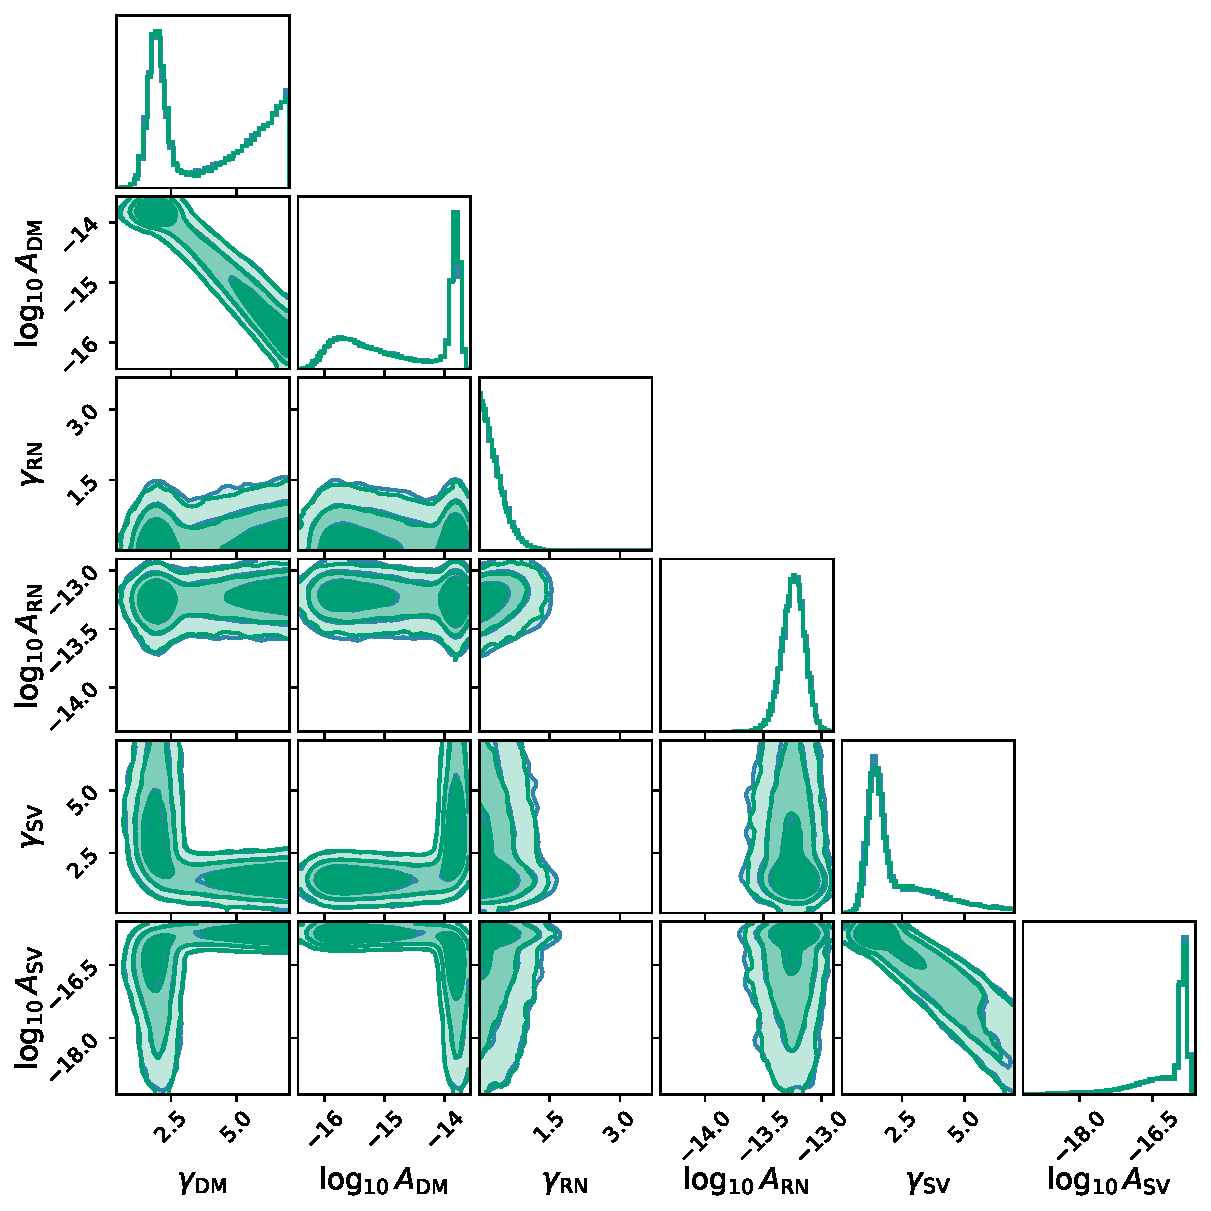
\includegraphics[width=0.75\textwidth]{Figure/cap5/01_discovery_vs_enterprise.pdf}
    \caption{Posterior distributions of the six noise parameters of
    PSR~J1640+2224 obtained from the DR2low data with \textsc{Discovery}
    (blue) and with \textsc{Enterprise} (green). The contours enclose $68\%$,
    $95\%$ and $99.7\%$ of the probability.}
    \label{fig:disc_vs_ent}
\end{figure}

\subsection{DR2low and DR2new+} \label{sec:dr2new}

To show the role of the low radio frequencies, we repeat the analysis on
the DR2new+ dataset, which contains only the observations of the EPTA
telescopes at 1.3--2.6\,GHz, without the LOFAR data. The noise model, the
number of Fourier components and the priors are the same used for DR2low.

The two posterior distributions are compared in
Figure~\ref{fig:dr2low_vs_dr2new}. With DR2new+ none of the parameters of
the chromatic processes is constrained. The posteriors of
$\gamma_{\rm DM}$ and $\gamma_{\rm SV}$ cover the whole prior range, and
those of the amplitudes extend from the lower bound of the prior up to
$\log_{10}A \simeq -13$, so that the data only exclude the largest
amplitudes. The same happens for the intrinsic red noise. In the band of
DR2new+ the chromatic factor of Eq.~\eqref{eq:chrom} is of order one for
both chromatic processes, so they are hard to distinguish from the
achromatic red noise and from each other.

With DR2low the posteriors are much narrower. The LOFAR observations are
at radio frequencies about ten times lower, where the DM variations and
the scattering variations are much stronger and depend on $\nu$ in
different ways, and this allows the chromatic processes to be separated
from the achromatic red noise. The amplitude of the intrinsic red noise,
for example, is unconstrained with DR2new+, while with DR2low it is
$\log_{10}A_{\rm RN} = -13.24^{+0.09}_{-0.10}$. A good coverage in radio
frequency is therefore necessary to measure the chromatic noise of this
pulsar.

\begin{figure}[H]
    \centering
    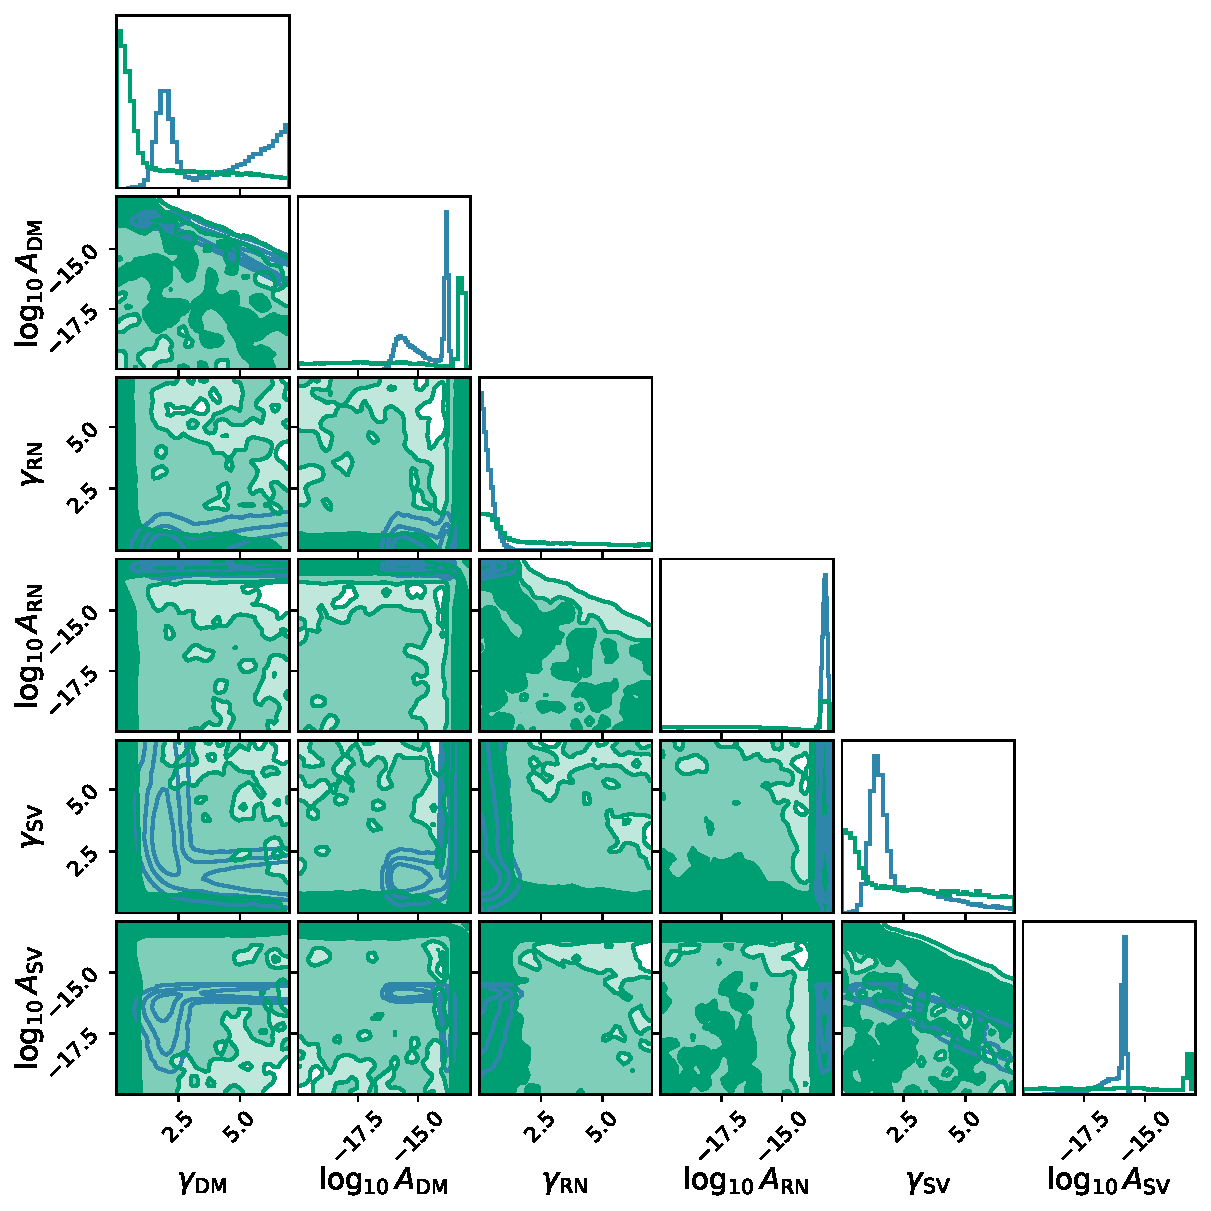
\includegraphics[width=0.75\textwidth]{Figure/cap5/02_DR2low_vs_DR2newplus.pdf}
    \caption{Posterior distributions of the six noise parameters of
    PSR~J1640+2224 obtained from the DR2low data (blue) and from the DR2new+
    data (green). The contours enclose $68\%$, $95\%$ and $99.7\%$ of the
    probability.}
    \label{fig:dr2low_vs_dr2new}
\end{figure}

\subsection{The DM--scattering degeneracy} \label{sec:degenerazione}

We now look in more detail at the DR2low posterior of
Figure~\ref{fig:disc_vs_ent}. The intrinsic red noise is well constrained
and its posterior has a single peak. The DM variations behave differently.
The posteriors of $\gamma_{\rm DM}$ and $\log_{10}A_{\rm DM}$ have two
peaks, one at high amplitude and low spectral index,
$\log_{10}A_{\rm DM} \simeq -13.8$ and $\gamma_{\rm DM} \simeq 2$, and one
at low amplitude, $\log_{10}A_{\rm DM} \simeq -15.5$, where
$\gamma_{\rm DM}$ grows up to the upper bound of the prior. The two peaks
have a comparable weight, so the data do not clearly prefer one of them.
For this reason the median of $\gamma_{\rm DM}$ quoted in
Section~\ref{sec:validazione} falls between the two peaks.

The two peaks are related to the scattering parameters. In the panels that
combine a DM parameter with a scattering parameter the contours are not
ellipses but have the shape of an L. Along one arm the DM variations have
a high amplitude and the scattering is poorly constrained, with a tail
that extends to very low amplitudes. Along the other arm the scattering is
well constrained, $\log_{10}A_{\rm SV} \simeq -15.9$ and
$\gamma_{\rm SV} \simeq 1.4$, and the DM variations are weak. An L-shaped
posterior is the typical sign of a degeneracy between two processes. Each
arm corresponds to a case in which one of the two processes accounts for
most of the noise, while the other is compatible with zero. Here the
chromatic noise at low radio frequencies can be described either mostly
by the DM variations or mostly by the scattering variations, and the data
cannot choose between the two descriptions.

A posterior of the DM parameters with two peaks was also found for this
pulsar in the noise analysis of the DR2low dataset. The origin of this
structure is not known. A possible explanation is that the data contain a
noise process that is not included in the model, and that part of its
power is attributed to the DM variations. In Section~\ref{sec:sim} we
test this hypothesis with simulations.